% указываем класс документа
\documentclass[12pt,a4paper,openany]{extarticle}
% подключаем собственный стилевой файл 
\usepackage{mystyle}
% указываем язык (для автоматической вставки слов, типа "Глава", "Содержание", "Литература", "рис." и пр.
\selectlanguage{russian}
\graphicspath{{./images/}}
\usepackage[pdftex]{lscape}

\begin{document}

\part*{Лабораторная работа №5\\
Робот с дифференциальным приводом}

\section{Методические рекомендации}
\hspace*{\parindent}До начала работы студент должен выполнить предыдущие лабораторные этого цикла.

\section{Теоретические сведения}
\hspace*{\parindent}В прошлой работе вы успели познакомиться c таким приемом управления, как ПИД-регулятор. Путем его реализации вам удалось реализовать процесс движения вдоль стены с минимальной ошибкой управления. В данной лабораторной работе будет предложено созать алгоритм движения широко используемого робота с дифференциальным приводом в заданную точку. Такой вид конструкции робота предполагает достаточно большую подвижность и мобильность вкупе со сравнительно легкой математической моделью. В робототехнике широко применяется два способа локализации, т.е нахождения координат устройства.

\begin{itemize}  
\item Глобальный - получение абсолютных координат робота. Например, GPS 
\item Локальный - получение координат робота, относительно какой-либо точки. Например, центр комнаты.
\end{itemize}

В нашем случае модель робота EV3 будет работать в система координат, которая строится каждый раз заново в точке, где на роботе запускается программа. 

\paragraph*{Модель робота}$\phantom{-}$\\
\begin{figure}[h!]
	\centering{ 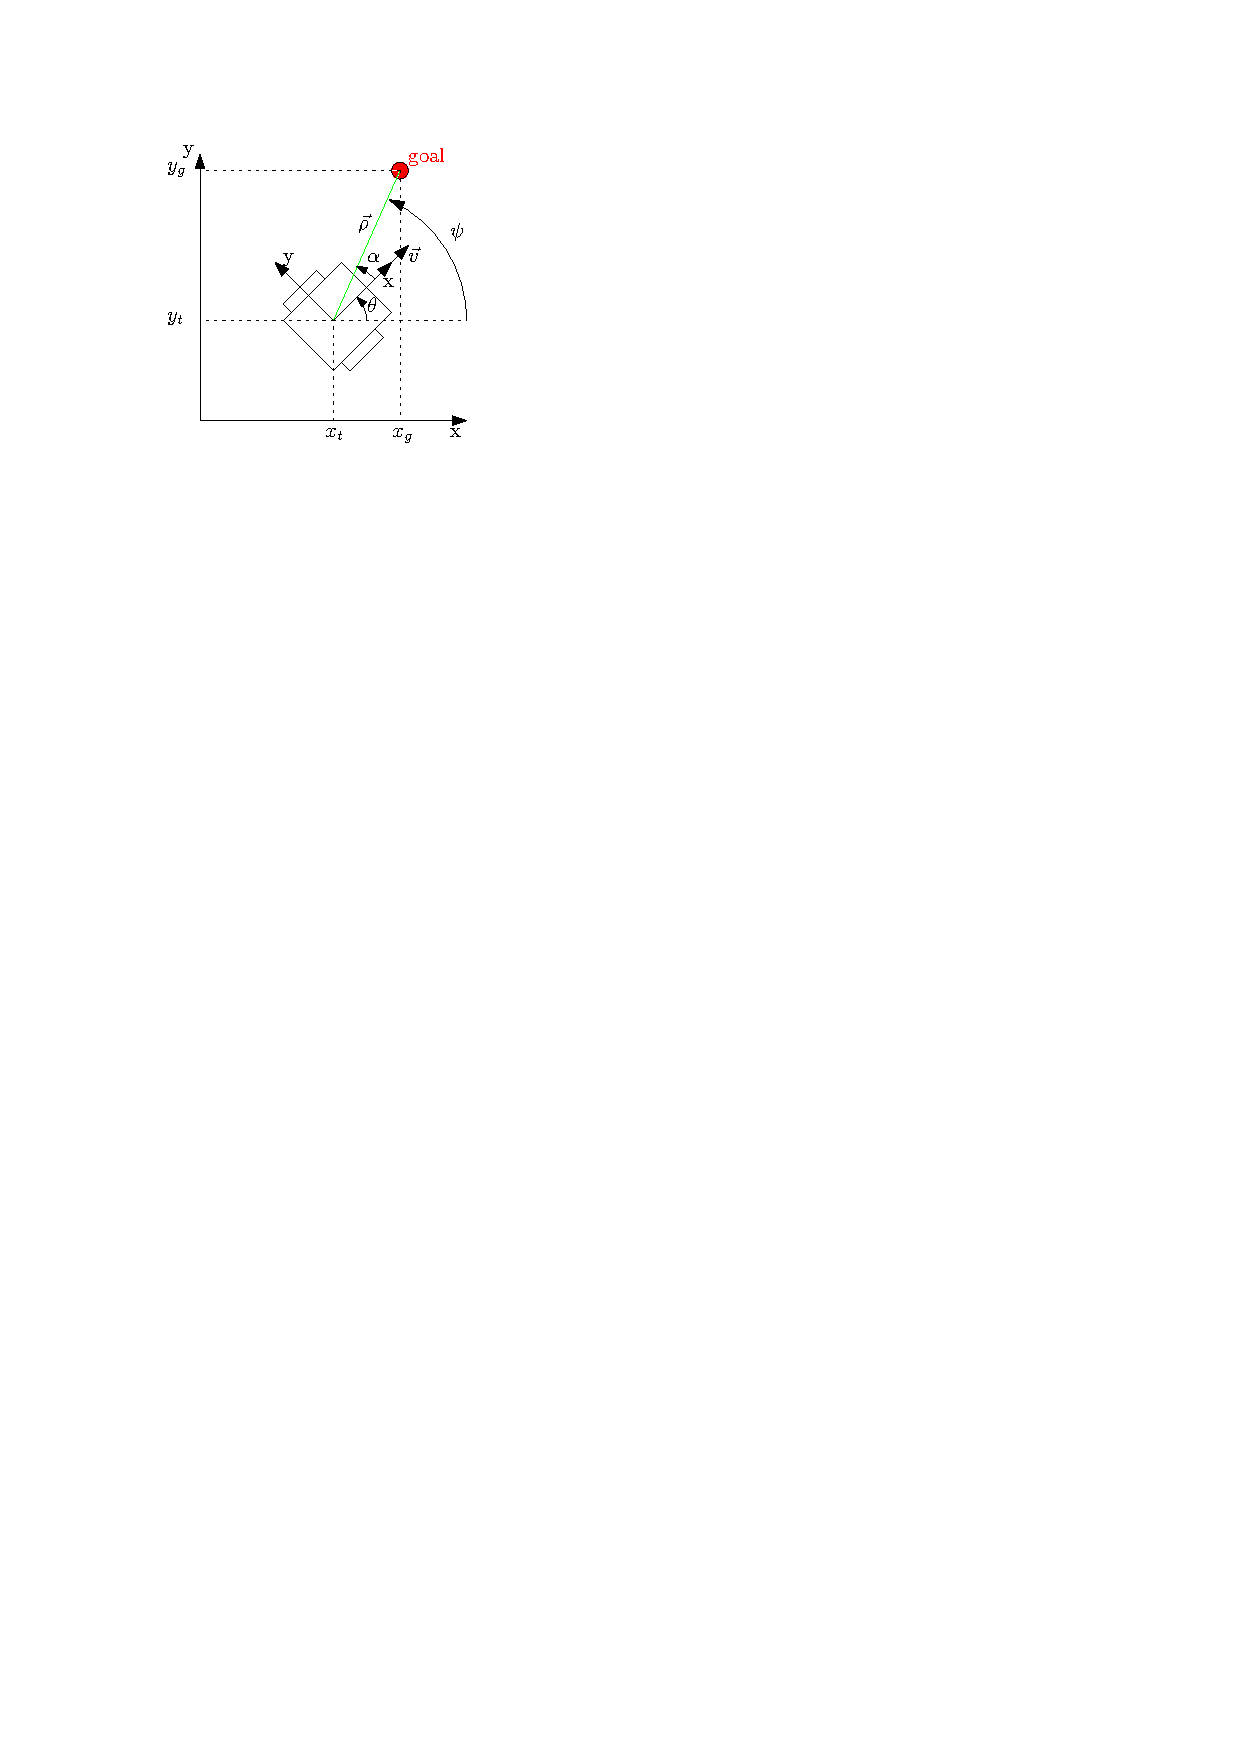
\includegraphics[width = 7cm]{model.pdf} }
	\vspace{1cm}
	\caption{Модель робота.}
	\label{fig:model}
\end{figure}

\hspace*{\parindent} Математическая модель, описывающая робота, всегда делится на две составляющие: динамическую и кинематическую. В динамической моделе учитываются всевозможные динамические показатели системы, такие как момент, сила и т.д. В кинематике рассматривается математика движения, без учета каких-либо сил. В данной работе мы рассмотрим только лишь кинематическую модель, что позволит нам углубиться в решение проблемы оптимального контроля.


Введем некоторые важные величины.
 
$\vec{p} = \begin{pmatrix}x_g - x_t & y_g - y_t\end{pmatrix}$- Расстояние от робота до целевой точки,

$\theta  = \arctan \frac{y_g - y_t}{x_g - x_t}$ - Угол между роботом и базовой осью ох (Курс)

$\psi = \arctan \frac{y_g}{x_g}$ - Угол между целевой точкой и осью ох (Азимут)

$\alpha = \psi - \theta$ - Курсовой угол. Разность между азимутом и курсом робота.

$\vec{v}$ - Линейная скорость робота.

Данная конструкция робота предполагает следующую систему уравнений, которая полностью описывает его движение:

\begin{equation}
 \begin{cases}
	\dot{x} = \cos{\theta} \cdot \frac{\omega_1 + \omega_2}{2}R\\
	\dot{y} = \sin{\theta} \cdot \frac{\omega_1 + \omega_2}{2}R\\
	\dot{\theta} = (\omega_1 - \omega_2)\frac{R}{B}
 \end{cases}
\end{equation}
где $\omega_1$,$\omega_2$ - угловые скорости колес, $R$ - радиус колеса, $B$ - Колесная база (расстояние между колесами)

Нетрудно заметить, что выражения $\frac{\omega_1+\omega_2}{2}R$ и $(\omega1-\omega2)\frac{R}{B}$ являются линейной и угловой скоростью робота соответсвенно. С учетом этого, перепишем выражение (1) в более приятный для глаз вид.
\begin{equation}
 \begin{cases}
	\dot{x} = \cos{\theta} \cdot V\\
	\dot{y} = \sin{\theta} \cdot V\\
	\dot{\theta} = \omega
 \end{cases}
\end{equation}
Ниже сформулируем формулы для контроля оптимальных линейной и угловой скорости робота. Заметим, что на данный момент происходит реализация лишь пропорционального регулятора и в будущих лабораторных работах к нему будет добавлена интегральная и дифференциальная составляющая.
\begin{equation}
 v = K_f \cdot p \cdot \cos{\alpha}, K_f > 0
\end{equation}
\begin{equation}
 \omega = K_r \cdot \alpha, K_r > 0
\end{equation}	
\end{document}

где $K_f$ и $K_p$ - коэффициенты для пропроцианального регулятора.
